\hypertarget{grundzuxfcge-der-industrierelevanten-vertruxe4ge}{%
\section{Grundzüge der industrierelevanten
Verträge}\label{grundzuxfcge-der-industrierelevanten-vertruxe4ge}}

\hypertarget{vertragstypen-uxfcbersicht}{%
\subsection{Vertragstypen Übersicht}\label{vertragstypen-uxfcbersicht}}

\begin{longtable}[]{@{}llll@{}}
Veräusserung & Gebrauchsüberlassung & Arbeitsleistung &
Übrige\tabularnewline
\endhead
Kaufvertrag & AirBnB & Werkvertrag & Lizenzverträge\tabularnewline
& Darlehen & Arbeitsvertrag &\tabularnewline
& Mietvertrag & Auftrag &\tabularnewline
\end{longtable}

\hypertarget{arbeitsvertrag}{%
\subsection{Arbeitsvertrag}\label{arbeitsvertrag}}

\begin{itemize}
\tightlist
\item
  Verrichtung von Arbeit nach Weisungen des Arbeitgebers
\item
  Risiko liegt beim Arbeitgeber
\end{itemize}

\hypertarget{werkvertrag}{%
\subsection{Werkvertrag}\label{werkvertrag}}

\begin{itemize}
\tightlist
\item
  Die Pflicht für einen Auftraggeber ein Werk zu erstellen (bspw.
  Software)
\item
  Das Entscheidende bei einem Werkvetrag ist das Resultat
  -\textgreater{} Erfolgsverschulden
\end{itemize}

\begin{figure}
\centering
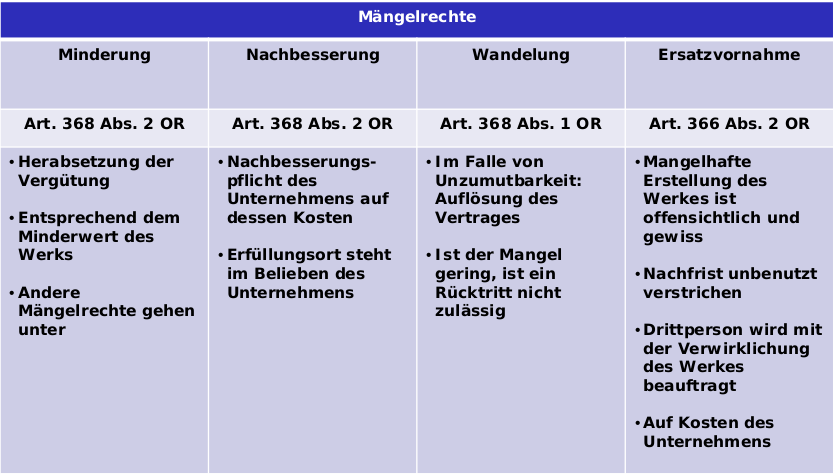
\includegraphics{figures/maengelRechte.png}
\caption{Mängelrechte Werkvertrag}
\end{figure}

\textbf{Ersatzvornahme}:\\
Wird ein Meilenstein während dem laufenden Werkvertrag nicht erreicht,
muss zuerst eine angemessene Nachfrist vereinbart werden. Wird diese
Nachfrist nach wie vor nicht genutzt und verstrichen, kann ein
Dritt-Unternehmen zur Lösung des Problems angestellt werden und die
Kosten müssen durch den Werkvertrag-Nehmer übernommen werden.

Drei Dinge, die bei einem Werkvertrag als erstes beachtet werden
sollten: - Zwischen wem ist der Vertrag? - Welches Recht und welcher
Gerichtsstand gilt? - Wie komme ich wieder aus dem Vertrag raus?

\hypertarget{preisvereinbarung}{%
\subsubsection{Preisvereinbarung}\label{preisvereinbarung}}

\begin{itemize}
\tightlist
\item
  \textbf{Pauschalpreis}: Vertraglich fixierter Betrag als Höchst- und
  Mindestpreis
\item
  \textbf{Globalpreis}: Festpreis (Teuerung angepasst)
\item
  \textbf{Ausnahme}: Missverhältnis zwischen Leistung und Vergütung\\
  Keine Voraussehbarkeit der Umstände.
\end{itemize}

\hypertarget{fehlende-preisvereinbarung}{%
\paragraph{Fehlende
Preisvereinbarung}\label{fehlende-preisvereinbarung}}

\begin{itemize}
\tightlist
\item
  Wert der Arbeit und der Aufwendungen sind füride Vergütungsbemessung
  masgebend (z.B. unverbindlicher Kostenvoranschlag). Ein solcher
  Kostenvoranschlag hat eine gewisse Bedeutung
\item
  zB «unverbindliche Kostenvoranschlag»
\item
  Damit das Kostenrisiko nicht ganz auf den Besteller übergeht, hat die
  «\textbf{unverbindliche Kostenvoranschlag}» doch eine gewisse
  Bedeutung
\item
  Achtung: Art. 375 Abs. 1 OR: Rücktrittsrecht des Bestellers, wenn
  «wesentlich» überschritten. (wesentlich = 10\%)
\end{itemize}

\hypertarget{pflichten-des-unternehmners-resp.-bestellers}{%
\subsubsection{Pflichten des Unternehmners resp.
Bestellers}\label{pflichten-des-unternehmners-resp.-bestellers}}

\textbf{Pflichten des Unternehmers} - Pflicht zur Herstellung eines
Werks (Art. 363 OR) - Materielles Werk: bewegliche oder unbewegliche
Sache - Geistiges Werk: wissenschaftliche oder künstlerische Leistungen
- Pflicht zur Lieferung des Werks (Art. 367 OR) - Erfolg geschuldet:
Resultat muss nach obj. Kriterien überprüft und als richtig oder falsch
qualifiziert werden können - keine besonderen Treuepflichten

\textbf{Pflichten des Bestellers} - Pflicht zur Annahme und Abnahme des
Werks (Art. 370 OR) - Werkmangel: Vertragliche zugesicherte
Eigenschaften fehlen - Wertqualität: normale Beschaffenheit -
Gebrauchsqualität: normale Benutzung - Prüfungspflicht innert nützlicher
Frist, ansonsten Genehmigungsfiktion! - Pflicht zur Leistung einer
Vergütung (Art. 363 u. 372 OR)

\hypertarget{auftrag}{%
\subsection{Auftrag}\label{auftrag}}

\begin{itemize}
\tightlist
\item
  Kein Erfolg garantiert
\item
  Sorgfältige Ausführung
\end{itemize}

Der Auftrag muss persönlich ausgeführt werden. Andernfalls musst der
Beauftragte den Auftraggeber informieren, falls die ausführende Person
wechselt.

\begin{figure}
\centering
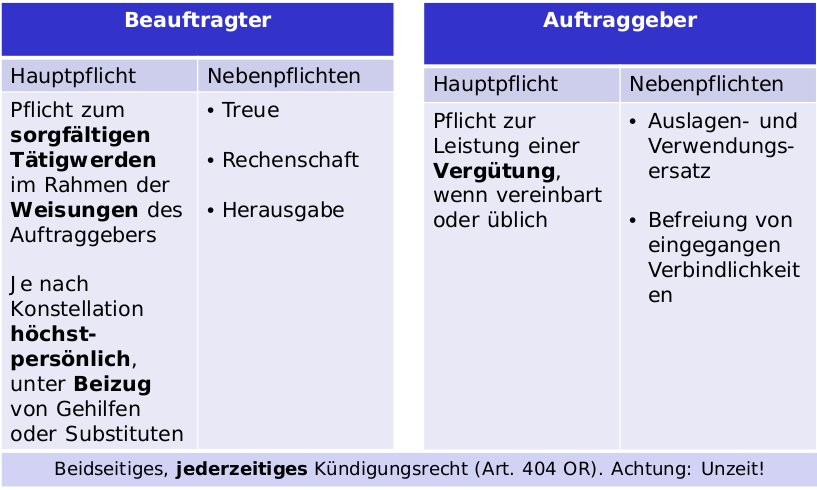
\includegraphics{figures/auftraggeberBeauftragter.png}
\caption{Beauftragter und Auftraggeber}
\end{figure}

\textbf{Herausgabe} bedeutet hier, dass der Arzt z.B. die Dossiers an
einen neuen Arzt weitergibt oder Informationen zur Verfügung stellt.\\
\textbf{Unzeit} bedeutet, dass die Gegenseite nicht mehr disponieren
kann.\\
\textbf{Kündigen} lässt sich ein Auftrag jederzeit von beiden Parteien,
\textbf{unabhängig davon ob Kündigungsfristen im Auftrag stehen} oder
nicht.

\hypertarget{vertragsabschluss}{%
\subsection{Vertragsabschluss}\label{vertragsabschluss}}

\hypertarget{voraussetzungen}{%
\subsubsection{Voraussetzungen}\label{voraussetzungen}}

\begin{enumerate}
\def\labelenumi{\arabic{enumi}.}
\tightlist
\item
  Rechts- und Handlungsfähigkeit der Vertragsparteien
\item
  Vorliegen beidseitigen Geschäftswillen
\item
  Austausch übereinstimmender Willenserklärungen Antrag:

  \begin{itemize}
  \tightlist
  \item
    Zeitlich erste Willenserklärung bei Vertragsverhandlung
  \item
    Muss alle für den Vertrag massgebenden Punkte enthalten\\
    Annahme:
  \item
    Zeitlich zweite Willenserklärung bei der Vertragsverhandlung
  \item
    Antragsempfänger erklärt Willen zum Vertragsabschluss durch die
    Annahme
  \item
    Inhaltliche Übereinstimmung von Antrag und Annahme notwendig
  \end{itemize}
\item
  Einhaltung von Formvorschriften, sofern erforderlich\\
  Gewisse Verträge müssen z.b. schriftlich, öffentlich oder beurkundet
  werden.
\item
  Keine Verletzung inhaltlicher Schranken / keine Willensmängel (Art.
  19/20ff. OR)
\end{enumerate}

\hypertarget{formvorschriften}{%
\subsubsection{Formvorschriften}\label{formvorschriften}}

\begin{figure}
\centering
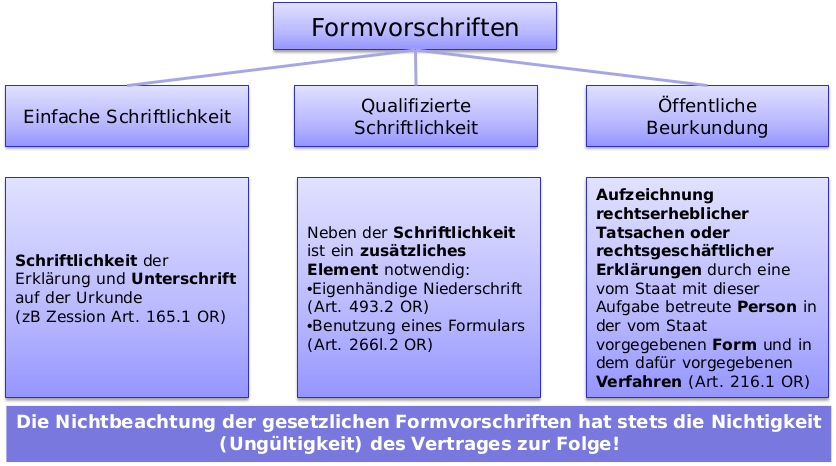
\includegraphics{figures/formvorschriftenVertragsabschluss.png}
\caption{Formvorschriften Vertragsabschluss}
\end{figure}

Ein Mail entspricht nicht \textbf{einfacher Schriftlichkeit}.\\
Ein Testament muss z.B. handschriftlich (Qualifizierte Schriftlichkeit)
sein, sonst ist es form-nichtig.\\
Eine Kündigung eines Mietverhältnisses durch den Vermieter muss mit
einem offiziellen Formular gemacht werden (Qualifizierte
Schriftlichkeit).

\hypertarget{vertragserfuxfcllung}{%
\subsubsection{Vertragserfüllung}\label{vertragserfuxfcllung}}

\begin{itemize}
\tightlist
\item
  Bei der Vertragserfüllung werden die durch den Vertragsabschluss
  begründeten Obligationen (Verpflichtungen) erfüllt.
\item
  Das Internet ist ein neues Kommunikationsmedium, das heute vermehrt
  dazu benutzt, übereinstimmende Willensäusserungen auszutauschen, die
  zu Vertragsabschlüssen führen (Art. 1 OR).
\item
  Fragen des Vertragsabschlusses und der Vertragserfüllung regeln sich
  -- genau wie beim mündlichen Vertragsabschluss oder beim brieflichen
  Austausch von Willenserklärungen -- nach den allgemeinen Bestimmungen
  des Obligationenrechts.
\end{itemize}

\hypertarget{vertragsverletzungen}{%
\subsubsection{Vertragsverletzungen}\label{vertragsverletzungen}}

\begin{figure}
\centering
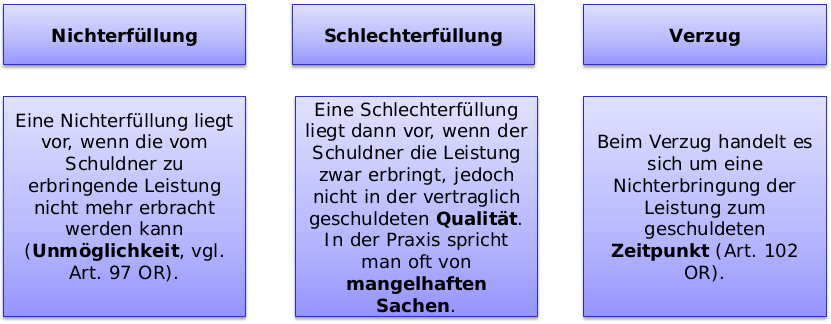
\includegraphics{figures/agbVertragsverletzungen.png}
\caption{AGB Vertragsverletzung}
\end{figure}

\textbf{Knonentionalstrafe:} Ist unabhängig ob wirklich ein Schaden
entstanden ist oder nicht. Zudem kann zusätzlich die Vertragserfüllung
trotzdem verlangt werden.

\hypertarget{agb}{%
\subsection{AGB}\label{agb}}

AGB sind \textbf{vorformulierte} Vertragsbestimmungen, die als Grundlage
für eine Vielzahl von Verträgen verwendet werden, die der Verfasser mit
seinen Kunden schliesst.

Ziele von AGB: - \textbf{Rationalisierungszweck} - Besserstellungszweck:
- Freizeichnungs-Klauseln - Sicherheiten-Klauseln - Risikoverlagerungen
- Verhandlungsvorgabe

\hypertarget{einbezug}{%
\subsubsection{Einbezug}\label{einbezug}}

Für das Zustandekommen eines Vertrages (Konsens) bedarf es der
übereinstimmenden gegenseitigen Willenserklärungen beider Parteien. Dies
gilt auch für die Einbeziehung der AGB in den Individualvertrag

\textbf{Voraussetzungen der AGB-Einbeziehung} - AGB-Kundbarmachung:
Kunde \textbf{ist vor oder während} der Vertragsverhandlungen auf die
AGB hinzuweisen - AGB-\textbf{Kenntnisnahme}: Kunde muss spätestens vor
Vertragsschluss Gelegenheit zur Kenntnisnahme haben Achtung:
Nachgeschobene AGB sind ungültig - AGB-Geltung: Kunde muss mit der
AGB-Geltung einverstanden sein

\hypertarget{typologisierung}{%
\subsubsection{Typologisierung}\label{typologisierung}}

\begin{figure}
\centering
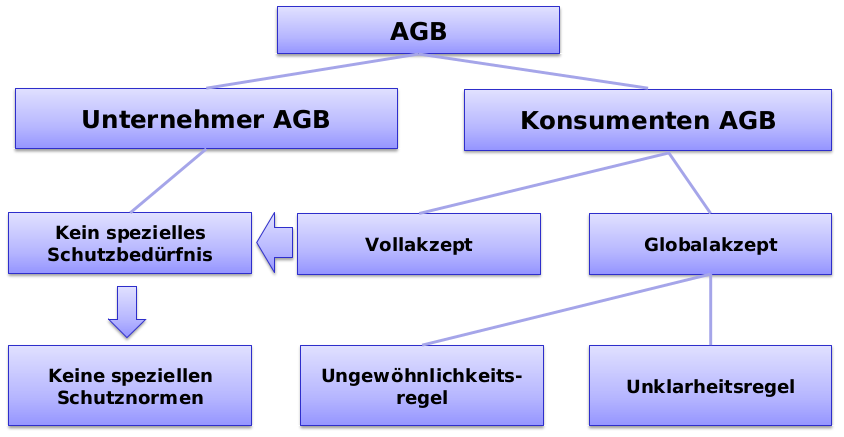
\includegraphics{figures/typolisierungAGB.png}
\caption{Typologisierung der AGB}
\end{figure}

\textbf{Globalakzept}: Bedeutet, dass viele leute einfach ohne zu lesen
die AGB akzeptieren. Dann gibt es die beiden folgenden Regeln zu
beachten.

\textbf{Vollakzept}: Bedeutet, wenn man bemerkt hat dass der Konsument
die AGB voll gelesen und akzeptiert hat.

\textbf{Ungewöhnlichkeits- und Unklarheitsregel}:\\
Verwendung missbräuchlicher Geschäftsbedingungen (Art. 8 UWG) „Unlauter
handelt insbesondere, wer allgemeine Geschäftsbedingungen verwendet, die
in \textbf{Treu und Glauben} verletzender Weise zum Nachteil der
Konsumentinnen und \textbf{Konsumenten} ein erhebliches und
ungerechtfertigtes \textbf{Missverhältnis} zwischen den vertraglichen
\textbf{Rechten und Pflichten} vorsehen.``

\textbf{Ungewöhnlichkeitsregel}: Enthalten AGB Bestimmungen, mit denen
der Kunde (nach Treu und Glauben) nicht rechnen muss, so sind diese
Bestimmungen für den Kunden nicht verbindlich\\
\emph{z.B. in einem Ski-Hüttchen der Gerichtsstand in Floria}

\textbf{Unklarheitsregel}: Finden sich in den AGB Regelungen, die unklar
sind, so werden diese zu Lasten des Verfassers der AGB ausgelegt\\
\emph{Wenn der Leser etwas der AGBs nicht versteht (oder verstehen
kann), werden diese Teile zu Lasten des Verfassers ausgelegt.}

\hypertarget{sia-vertruxe4ge}{%
\subsection{SIA-Verträge}\label{sia-vertruxe4ge}}

\begin{itemize}
\tightlist
\item
  Vertragsformulare der SIA für Geschäftsbeziehungen zwischen

  \begin{itemize}
  \tightlist
  \item
    \textbf{Bauherren und Planern} (Aufträge) sowie zwischen

    \begin{itemize}
    \tightlist
    \item
      BSP: Vertrag für Ingenieurleistungen Nr. 1003
    \end{itemize}
  \item
    \textbf{Bauherren und Unternehmern} (Werkverträge)

    \begin{itemize}
    \tightlist
    \item
      BSP: Werkvertrag Nr. 1023
    \end{itemize}
  \end{itemize}
\item
  Sicherstellung der \textbf{korrekten Einbindung} der entsprechenden
  Vertragsnorm
\item
  \textbf{Breit abgestützte Grundlage} für die Geschäftsbeziehung
\item
  Schweizweit anerkannt und für \textbf{80\% der Fälle als Standard
  anwendbar}
\item
  Knappe und \textbf{klare Struktur} / detaillierte Aspekte mithilfe von
  Beilagen
\end{itemize}

\hypertarget{swico-vertruxe4ge}{%
\subsection{SWICO-Verträge}\label{swico-vertruxe4ge}}

\begin{itemize}
\tightlist
\item
  IT-Modellverträge, welche durch Anwälte der Verbände SWICO und
  SwissICT erarbeitet werden
\item
  Faire und ausgewogene Regelungen
\item
  Konkrete Bezugnahme auf IT-relevante Vertragsgestaltungen
\item
  Nur Geltung, wenn konkret im Vertrag vereinbart
\end{itemize}

Vorteile Swico-Verträge: 1. Branchenbezogenheit 2. Fachgerechte
Formulierung
